\documentclass{cuxarticle}
\begin{document}
% タイトル
\begin{titlepage}
  \begin{titlepage}
  \begin{center}
    {\large 2024年度 学士学位論文}\\
    \vspace{19\zh}
    {\Huge 環境情報のセンシングを用いた他者の\\環境評価を表現するロボットシステム}\\ % タイトル
    % {\Large ―サブタイトル―}\\ % サブタイトル(なければコメントアウト)
    \vspace{22\zh}
    \large{
      宮城大学 事業構想学群 価値創造デザイン学類\\
      感性情報デザインコース\\
      \vspace{1\zh}
      22120165\\ % 学籍番号
      中村 龍造\\ % 著者
      \vspace{3\zh}
      指導教員 佐藤 弘樹 准教授
    }
  \end{center}
\end{titlepage}

\end{titlepage}
% アブスト
\begin{center}
  {\Large
    論 文 要 旨\\
    \vspace{2\zh}
    環境情報のセンシングを用いた他者の\\環境評価を表現するロボットシステム\\
    \vspace{2\zh}
  }
\end{center}

%   アブスト本文
本研究では、生活環境における他者の環境評価を表現するロボットシステムを提案する。我々は日常において、人間、動植物、モノなど多様な「他者」と共存している。他者はそれぞれ独自の感覚や基準で環境を評価しているが、我々がそれを直接知ることは難しい。本システムでは、環境センサーで取得したデータを他者基準で評価し、その評価結果をロボットの身体的動作を通じて表現する。「人間―本システム―外界」という関係を採用することで、従来の「人間―外界」という直接的な関係性を再構築し、相互理解の促進を目指す。

実装では、M5StickCによるセンシングとtoioロボットの動作制御を組み合わせ、人間(気温18-28℃)、猫(気温30-38℃)、バナナ(気温14-20℃、湿度45-85\%)、衣服(湿度65\%以下)など異なる他者の環境評価を表現するシステムを実装した。コンポーネント指向アーキテクチャを採用することで、システムの拡張性と保守性を確保し、「弱いロボット」のコンセプトを取り入れた動作表現により、ユーザーに自然な気づきを与えることを目指した。

検証の結果、「よたよた」とした「弱さ」を感じさせる動きの表現や、同一ロボットでの他者の識別性など、いくつかの課題が明らかになった。しかし、本システムは生活環境における多様な他者理解を支援する新たな手法として、人間と他者の相互理解を促進し、多様な存在と相互作用する生活空間の発展に貢献する可能性を示した。さらに介護シーン、遠隔ワーク環境、植物ケアなど具体的なユースケースへの応用可能性についても検討を行った。

\vspace{3\zh}

\begin{flushright}
  宮城大学 事業構想学群 価値創造デザイン学類 感性情報デザインコース\\
  22120165\\ % 学籍番号
  中村 龍造\\ % 著者
\end{flushright}

% 目次
\tableofcontents

\chapter{序論}

\section{研究背景}
我々は生活環境において、人間、動植物、モノなどの多様な「他者」と共存している。他者はそれぞれ独自の感覚や基準で世界を認識しており、我々がそれを直接知ることはできない。近年、脱人間中心デザインの観点から、他者理解の重要性が指摘されている。しかしながら、他者の感覚や基準を共有することは難しく、生活環境における継続的な他者理解を支援する手法は十分に確立されていない。

同じ人間どうしであっても、個人差によって環境への評価や感覚には違いがある。このような状況において、生活空間に小さな存在が配置され、他者の感覚を代弁することで、私たちの生活をより豊かにする可能性がある。

\section{関連研究}

\subsection{他者視点の表現}
他者視点の表現に関する取り組みとして、次の2つの事例を挙げる。

\subsubsection{In the Eyes of the Animal}
In the Eyes of the Animal\cite{--EyesAnimal}は、動物の環世界(Umwelt)を通して森林環境を体験するVRを用いた没入型作品である。このプロジェクトでは、森林に生息する生物の知覚システムを通して環境を探索することができる。ユクスキュルが提唱した「環世界(Umwelt)」の概念に基づき、各生物種が独自の感覚能力と認知特性によって形成する主観的な知覚世界を表現している。

本事例はVR体験に限定されており、実際の生活環境で、継続的に他者理解を支援することは困難である。また動物の知覚を一時的な没入体験としてのみ提示しており、長期的な相互作用の可能性については考慮されていない。

\subsubsection{rapotosis}
衣服における他者表現の事例としては、rapotosis\cite{--ソンヨン}が挙げられる。本事例では、ロボットやwebサービスを用いて、一定期間使用されていない衣服が自律的に「自殺」するプロセスを表現している。具体的な実装としては、ハンガーから服が自動的に落下する装置や、衣服がSNSを通してユーザにメッセージを送信する機能。所有者の同意を得た後に自動的に出品される仕組みや、新しい所有者が決まると自走するダンボールで回収されるシステムから構成される。

本事例では表現対象が特定の衣服という限定的な対象にのみ焦点を当てており、より広範な他者の感覚表現には至っていない。

\subsection{環境センシング}
環境センシングシステムでは、個々人基準の環境評価の重要性が示されている\cite{Saini-2020-IndoorAirQualityMonitoring}。環境センシングシステムは、湿度、CO2、CO、PM2.5、VOCsなどの環境パラメータを測定し、居住環境の質を継続的に監視する。しかし、これらの情報はアプリケーションの視覚的UIを通じて一方的に表示されることが多く、利用者とシステム間の双方向的なインタラクションや、身体的動作による環境情報の表現と理解を促す事例は限られている。また、多くの既存システムは実験室や管理された環境で評価されており、実際のフィールド環境におけるIAQパラメータの信頼性の高い意思決定、評価、測定に課題が残る。

\subsection{HRIの先行事例}
本研究に関連するロボットインタラクションの先行事例として、次の2点を挙げる。

\subsubsection{HERMITS}
HERMITS\cite{--HERMITSProceedings33rdAnnual}は、同一の自走式ロボットに対して「シェル」と呼ばれる外装を切り替えることで、異なる機能を提供する試みである。これらのシェルはロボットの移動能力を利用して動的に再構成される。HERMITSのアプローチはシンプルなロボットを用いて、多様な相互作用機能をもたらす新しいTUIの可能性を示している。

本研究では、この考え方をソフトウェア的に実装し、同一のロボットハードウェアで多様な「他者」を表現することを目指した。

\subsubsection{弱いロボット}
岡田らの提案する「弱いロボット」\cite{岡田-2017-弱いロボ}は、あえて「弱さ」を表現する動作をデザインすることで、人間を積極的にタスク遂行に取り入れるロボットである。ロボットの完全性や自律性を追求するのではなく、むしろ「不完全さ」や「弱さ」を意図的にデザインに取り入れることで、人間との関係性を強化することを狙っている。例えば、「ゴミ箱ロボット」\cite{岡田美智男-2012-ゴミ箱ロ}は一人ではゴミを拾えないが、子どもたちのアシストを引き出すことで結果的にゴミを収集できる。また「Talking-Ally」\cite{岡田美智男-2012-ゴミ箱ロ}は会話の中で言い淀みや言い直しを活用し、聞き手と相互に会話の調整を行う。これらのロボットは「個体」としての能力を抑制しながらも、周囲との「関係」を通じて豊かな相互作用を生み出している。本研究では、この「弱さ」の表現を取り入れ、自然な形で人間の注意を喚起する手法を検討した。

\section{研究目的}
本研究では、生活空間における他者の環境評価を表現するロボットシステムを提案する。センサーで取得した環境データを他者基準で評価し、その評価結果をロボットの身体的動作を通じて表現する。生活空間にロボットを分散配置することで、継続的に他者を表現し続けることを目指す。また、他者の表現手段を身体的動作とすることで、同一のロボットで多様な他者表現を可能とする。

図\ref{fig:system-concept}のような、身の回りで他者の感覚を代弁する小型ロボットが活動するシステムを実装することで、人間と他者の相互理解を促進し、多様な存在が共存する生活空間の実現に貢献する。

\begin{figure}[h]
  \centering
  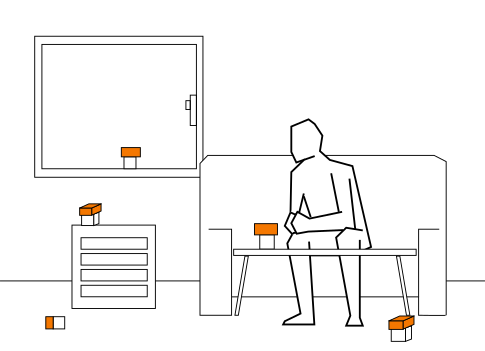
\includegraphics[keepaspectratio,height=0.2\textheight]{resources/robot-in-house.png}
  \caption[short]{本システムの構想図。\\生活空間に分散配置された小型ロボットが他者の感覚を代弁する。}
  \label{fig:system-concept}
\end{figure}

\chapter{提案システム}

\section{システム要件}
研究目的を踏まえ、本システムの要件として以下の3点を設定した

\begin{enumerate}
  \item 生活環境で継続的に他者の環境評価を表現できること
  \item 多様な他者を表現できること
  \item 特別な操作なしでの自然な他者理解を支援できること
\end{enumerate}

\section{システム構成}
本システムは以下の要素から構成される

\subsection{システム全体の構成}
本システムの全体処理フローは、以下の4つのフェーズから構成される。

\begin{enumerate}
  \item \textbf{センシングフェーズ}:環境センサーが環境データを取得し、ロボットシステムに送信する
  \item \textbf{評価フェーズ}:受信した環境データを「他者」個別の基準で評価し、環境に対する評価結果を出力する
  \item \textbf{アクション決定フェーズ}:評価結果に基づき、「他者」の状態を表現するアクションを決定する
  \item \textbf{実行フェーズ}:決定されたアクションをロボットに送信し、実行する
\end{enumerate}

このサイクルは継続的に実行され、環境の変化に応じてリアルタイムに「他者」の状態が表現される仕組みとなっている。システム全体のフロー図を図\ref{fig:system-flow}に示す。

\begin{figure}[h]
  \centering
  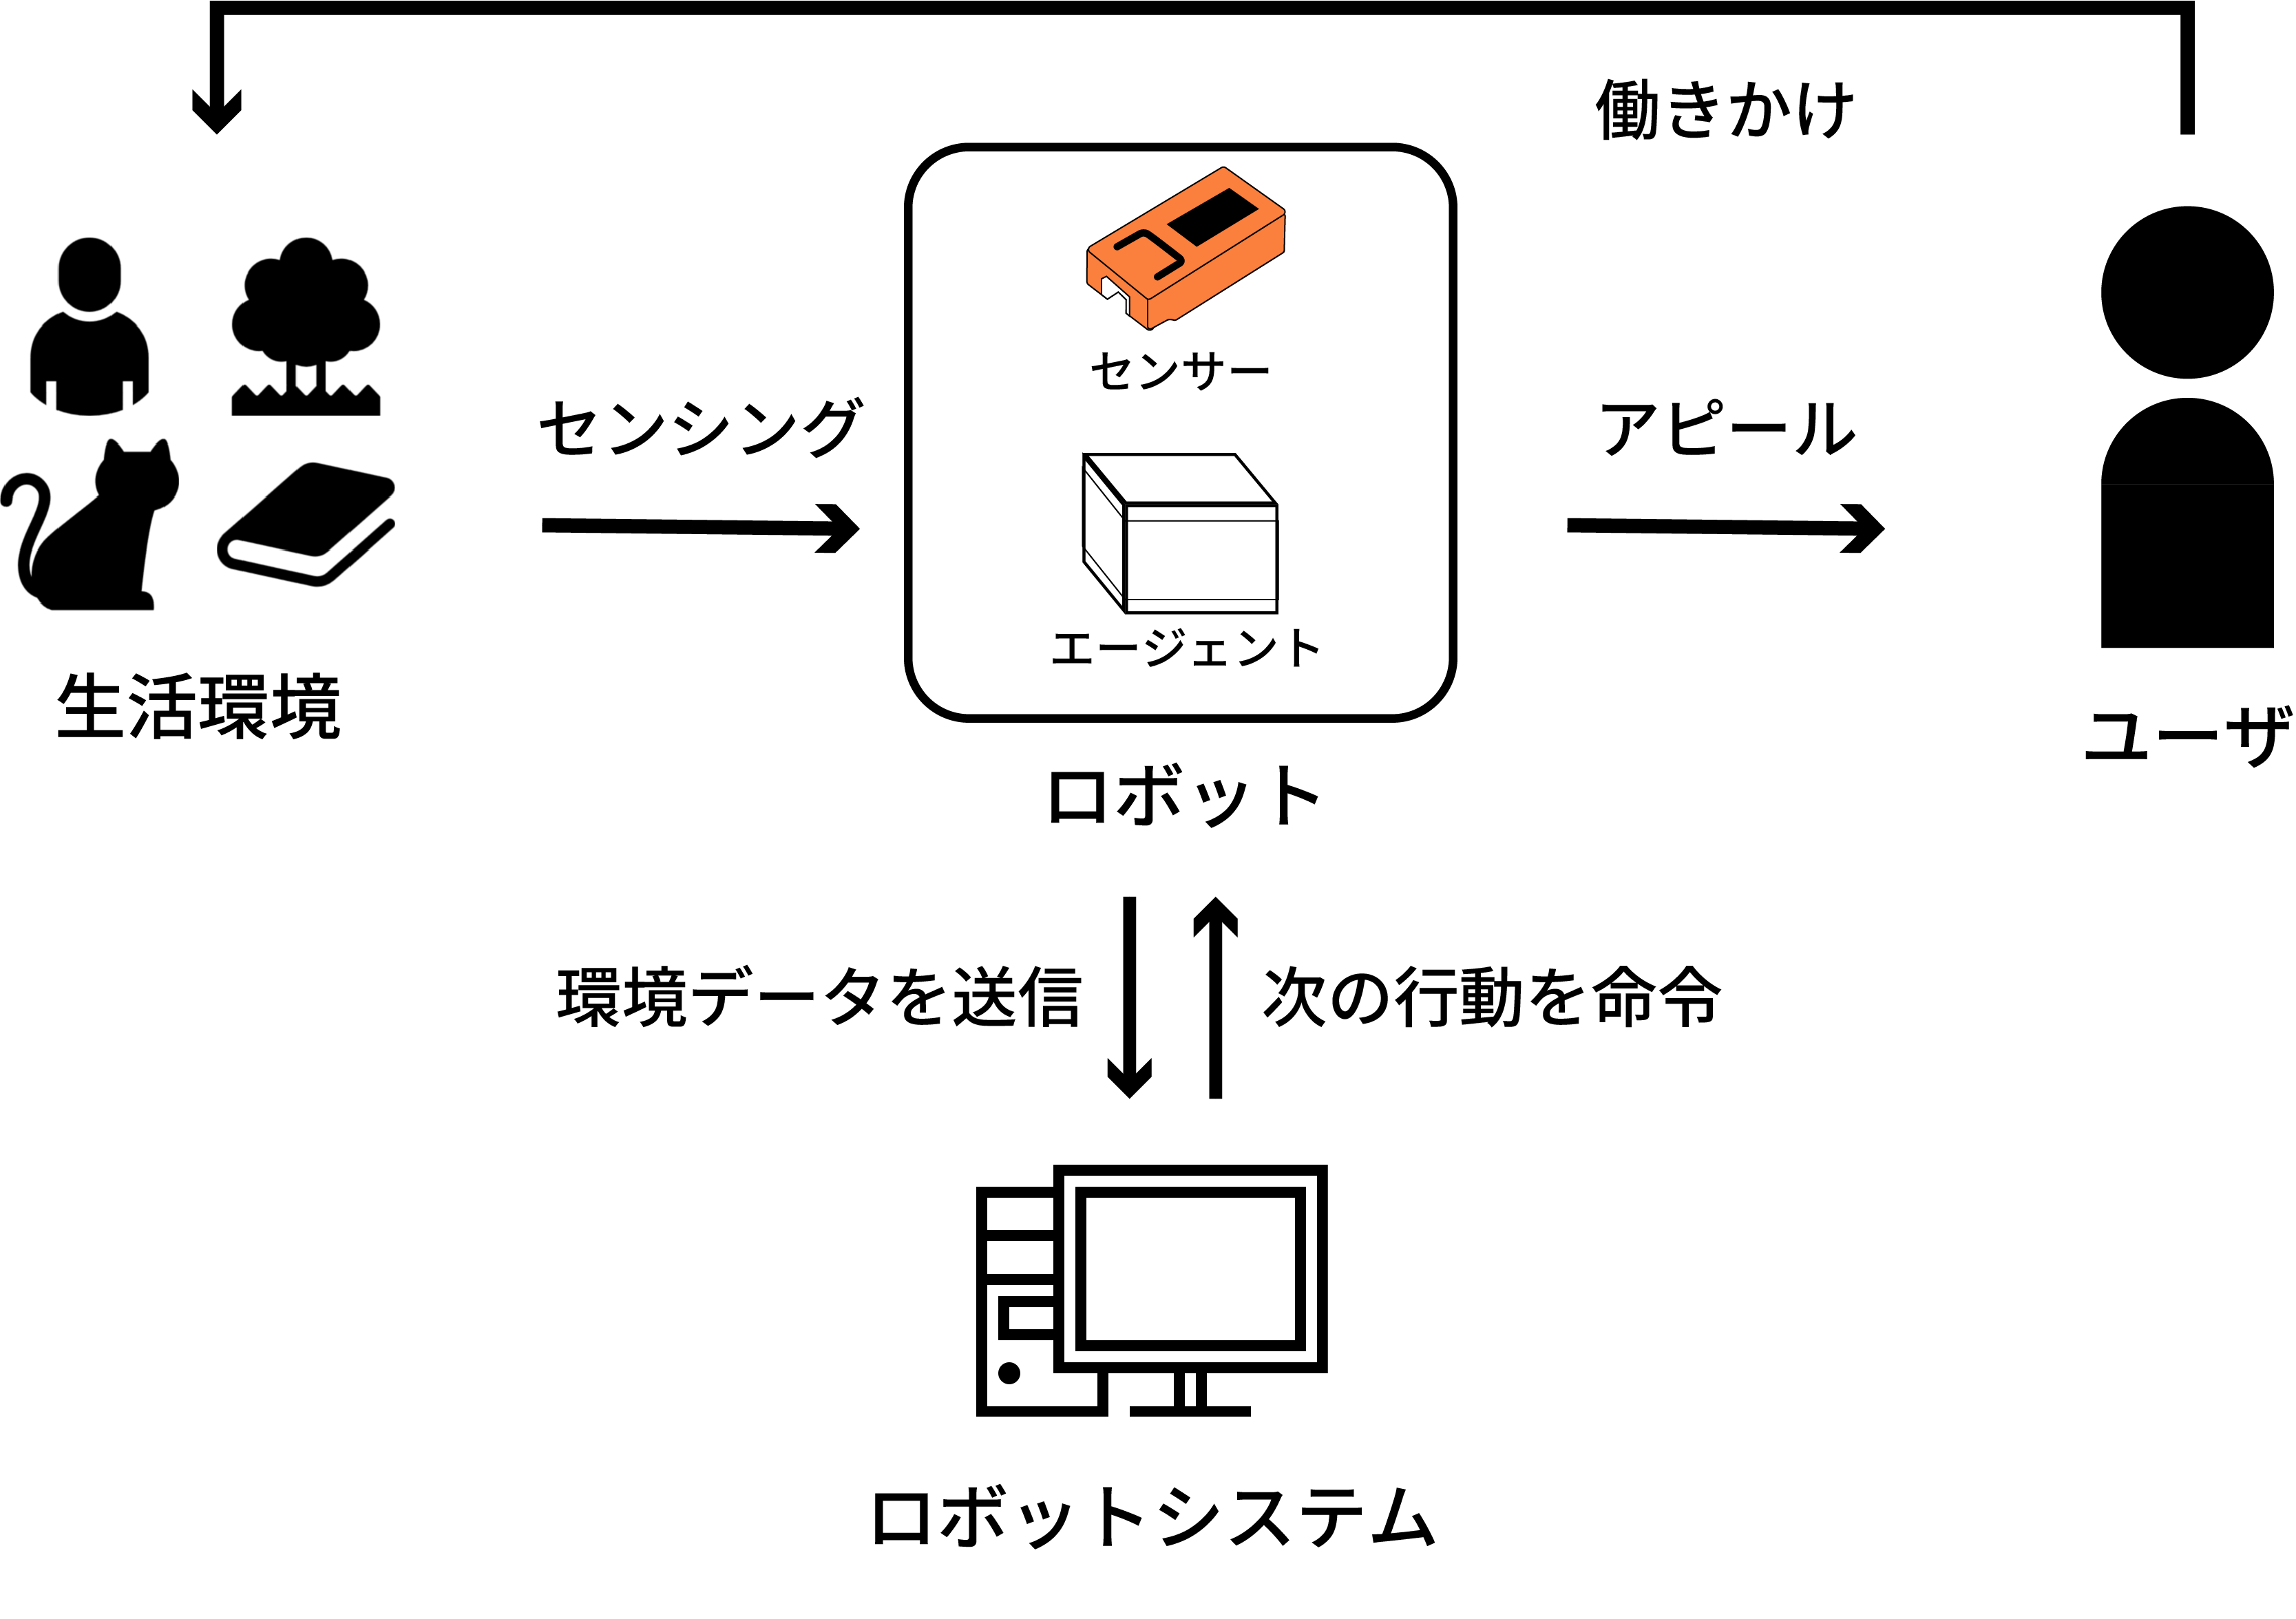
\includegraphics[keepaspectratio, height=0.3\textheight]{resources/system-flow.png}
  \caption[short]{システム全体のフロー図。センシングフェーズ、評価フェーズ、アクション決定フェーズ、実行フェーズの4つのフェーズから構成される。}
  \label{fig:system-flow}
\end{figure}

\subsection{ハードウェア構成}
本システムのハードウェアは、センシングユニットとエージェントロボットから構成される。センシングユニットは環境データの取得およびロボットシステムへの送信を行い、エージェントロボットはアクション決定フェーズで決定されたアクションを実行する。

\subsubsection{センシングユニット(M5StickC)}
本研究ではセンシングユニットとして M5StickC(M5Stack社)\cite{--M5StickC}を使用した。選定の主な理由は以下の技術的要因に基づく。

\begin{itemize}
  \item \textbf{スタンドアロン性能}:独立したマイクロコントローラとして機能し、外部PCなどに依存せずに長時間のセンシングが可能
  \item \textbf{高い拡張性}:複数のセンサーモジュールが使用可能であり、多様な環境データを対象としうる
  \item \textbf{コンパクトな形状}:小型・軽量であり、生活空間内の様々な場所に設置可能なほか、エージェントロボットへの積載が可能
  \item \textbf{無線通信}:Wi-Fi、Bluetoothなどの無線通信機能を内蔵し、システム内のデータ連携が容易
  \item \textbf{開発環境}:Arduino IDEやPlatformIOを用いた標準的な開発環境が整備されている
\end{itemize}

\subsubsection{エージェントロボット(toio)}
エージェントロボットにはtoio(SONY社)\cite{--小さなキ}を使用した。理由は次の技術的要件を満たしていたためである。

\begin{itemize}
  \item \textbf{位置認識能力}:専用マット上のパターン読み取りにより高精度な位置・方向認識が可能
  \item \textbf{マルチモーダルな表現能力}:移動、LEDによる色表現、音声出力など、複数のモダリティによる表現が可能
  \item \textbf{スケーラビリティ}:複数台を同時制御するスワームロボットとしての利用が可能
  \item \textbf{豊富な開発環境}:Unity、JavaScript、Pythonなど複数の開発言語やフレームワークとの互換性が高い
  \item \textbf{先行研究の存在}:HERMITS\cite{--HERMITSProceedings33rdAnnual}のような先行研究が存在し、TUI研究においての実績がある
\end{itemize}

\subsection{ソフトウェア構成}
システムは以下のモジュールで構成される:

\begin{enumerate}
  \item センシングシステム
    \begin{itemize}
      \item 環境データの取得
      \item Bluetooth通信(ボーレート:9600)
      \item PlatformIOを使用した開発環境
    \end{itemize}

  \item 評価システム
    \begin{itemize}
      \item 環境データと最適条件の差分を評価
      \item 評価スコアの生成
      \item Result構造体による評価結果の表現
    \end{itemize}

  \item アクション決定システム
    \begin{itemize}
      \item 評価結果に基づく動作パターンの決定
      \item ActionLibraryによる動作パターンの実装
      \item ロボットへの動作命令生成
    \end{itemize}

  \item ロボット制御システム
    \begin{itemize}
      \item Unity の toio SDK ライブラリによる実装
      \item 動作の実行と監視
    \end{itemize}
\end{enumerate}

\subsection{コンポーネント指向アーキテクチャ}
本システムは拡張性と保守性を考慮し、コンポーネント指向アーキテクチャを採用した。各機能をコンポーネントとして独立させることで、新しい「他者」や環境データの追加が容易になる設計となっている。

システムの各Cubeオブジェクトには以下のコンポーネントが追加される:

\begin{enumerate}
  \item SerialHundler:センサーとの通信を担当
  \item SensorComponent:環境データの取得と整形を担当
  \item EvaluateBase:取得データの評価を担当
  \item ActionGenerator:評価結果に基づいたアクション生成を担当
  \item Toio:ロボットの制御を担当
\end{enumerate}

このアーキテクチャにより、例えば新しい環境データ(CO2など)の追加や、新しい「他者」(人間以外の生物など)の追加が、既存のコードを変更することなく実現可能となっている。

\subsection{アクションライブラリと「弱いロボット」の動き}
本システムでは、「他者」の感覚を表現するためのアクションライブラリを実装した。基本モーションとして、移動(Translate)、回転(Rotate)、停止(Stop)、音声(Sound)、LED点灯(LED)などの機能を提供し、これらを組み合わせることで複雑な表現を可能にしている。

特に「弱いロボット」の特徴である「よたよた」とした動きを実現するため、微細な動きの組み合わせやテンポの調整を行った。例えば、短時間での方向転換や不規則な間隔での停止を組み合わせることで、ロボットが「必死に何かをしようとしているが、うまくいかない」印象を与える動きを実装した。

各「他者」(人間、猫、バナナ、服など)ごとに異なるアクションパターンを設計し、それぞれの「他者」が持つ特性や感覚を表現できるようにした。

\subsection{評価システムの詳細設計}
本システムの評価部分は、「他者」ごとの独自の基準で環境データを評価するよう設計されている。具体的には、Result構造体を用いて環境データの評価結果を表現している。このResultには以下の情報が含まれる:

\begin{enumerate}
  \item Score:環境データの評価スコア(適正値からの偏差)
  \item Unit:評価対象のデータ単位(°C、\%など)
  \item Message:評価結果に関する説明メッセージ
\end{enumerate}

例えば、猫の適温評価では、猫にとっての快適温度(30~38℃)を基準とし、現在の温度がこの範囲から外れるほど、正負のスコアが増加する設計となっている。このスコアは後述するアクション生成システムで、動作の種類や強度を決定するのに使用される。

同様に、服の湿度評価では、カビが発生しにくい湿度範囲(40~60\%)を基準とし、現在の湿度がこの範囲から外れるほどスコアが増加する仕組みとなっている。

\chapter{実装と評価}

\section{実装事例}
以下の4種の他者について実装を行った:

\subsection{人間}\cite{JianZhuWuHuanJingWeiShengGuanLiJiZhunnituite|HouShengLaoDongSheng}
\begin{itemize}
  \item 評価対象:気温(18-28℃)
  \item 動作パターン:
    \begin{itemize}
      \item 快適時:アピールなし
      \item 不快時(暑い/寒い):激しい動作
    \end{itemize}
\end{itemize}

\subsection{猫}\cite{stellaEnvironmentalAspectsDomestic2016}
\begin{itemize}
  \item 評価対象:気温(30-38℃)
  \item 動作パターン:
    \begin{itemize}
      \item 快適時:定点での回転
      \item 不快時:ランダムな往復動作
    \end{itemize}
\end{itemize}

\subsection{バナナ}\cite{--バナナの}
\begin{itemize}
  \item 評価対象:
    \begin{itemize}
      \item 気温:14-20℃
      \item 相対湿度:45-85\%
    \end{itemize}
  \item 動作パターン:3段階の状態表現
    \begin{itemize}
      \item 快適時:ゆっくりとした動作
      \item 不快時:ノロノロ動いて低音で鳴く
    \end{itemize}
\end{itemize}

\subsection{衣服}\cite{--クローゼ}
\begin{itemize}
  \item 評価対象:相対湿度(65\%以下)
  \item 動作パターン:
    \begin{itemize}
      \item 快適時:じっとする
      \item 不快時:不規則な動作と音によるアピール
    \end{itemize}
\end{itemize}

\section{実装した主体と環境データの組み合わせ}
本研究では、多様な「他者」とセンサーデータの組み合わせを実装した。表\ref{table:entities}に実装したパターンの概要を示す。

\begin{table}[htbp]
  \caption{実装した主体-センサー対応表}
  \label{table:entities}
  \centering
  \begin{tabular}{|l|l|l|l|}
    \hline
    主体 & センサー & 立ち位置 & アクション \\
    \hline
    人間 & 気圧 & 人間,気圧パターン & 偏頭痛.苦しそうに身体を振る \\
    \hline
    猫 & 気温 & 動物,気温パターン & 暑そうでイライラする \\
    \hline
    植物 & CO2 & 植物,CO2パターン & 元気になる(光合成) \\
    \hline
    バナナ & 気温,湿度 & ナマモノ,センサ複合パターン & 腐りそうになる \\
    \hline
    服 & 湿度 & 無機物,湿度パターン & カビることを不安がる動き \\
    \hline
  \end{tabular}
\end{table}

これらの組み合わせにより、本システムが人間、動物、植物、ナマモノ、無機物といった多様な「他者」の表現に対応可能であることを示している。特にバナナの例では、保存に適した14~20℃という特定の温度条件を持つ「他者」の表現も可能であることが確認された。

\section{センサーユニットの動作時間検証}
M5StickCベースのセンサーユニットについて、異なるセンサーモジュールごとの動作時間を検証した結果を表\ref{table:battery}に示す。

\begin{table}[htbp]
  \caption{センサーユニットの動作時間検証結果}
  \label{table:battery}
  \centering
  \begin{tabular}{|l|c|c|c|l|}
    \hline
    センサー構成 & 起動時間 & スリープ時間 & 画面輝度 & 備考 \\
    \hline
    M5StickC+ENV II & 57分 & 10秒 & 1 & 標準設定 \\
    \hline
    M5StickC+ENV II & 86分 & 30秒 & 0 & powerSaveOn使用 \\
    \hline
    M5StickC+CO2L & 38分 & 5秒 & 0 & 標準設定 \\
    \hline
    M5StickC+CO2L & 55分 & 30秒 & 0 & powerSaveOn使用 \\
    \hline
  \end{tabular}
\end{table}

これらの結果から、スリープ時間の延長と画面輝度の低減によって、バッテリー持続時間を最大約1.5倍に延長できることが確認された。理論上、さらにスリープ時間を延長することで最大6倍程度まで動作時間を延ばせる可能性があるが、環境データの変化を適切に捉えるサンプリングレートとのバランスを考慮する必要がある。

\section{評価結果}
実装したシステムの動作検証により、以下の3点の課題が明らかになった:

\begin{enumerate}
  \item 最適な環境の基準には個人差がある
    \begin{itemize}
      \item 対応策:リアルタイムに基準を調整可能なインタフェースの実装
    \end{itemize}

  \item 移動する他者はセンシング位置と他者の位置が一致しない
    \begin{itemize}
      \item 対応策:空間的な変化が小さい環境データを中心に評価
    \end{itemize}

  \item 時間経過で最適条件が変化する他者は、即時的な評価では表現しきることができない
    \begin{itemize}
      \item 対応策:環境データの長期記録と分析、それに伴う評価基準の調整
    \end{itemize}
\end{enumerate}

\section{技術的課題と限界}
本システムの開発・検証過程で明らかになった技術的課題と限界を以下に整理する:

\begin{enumerate}
  \item \textbf{通信の安定性}:Bluetooth通信に依存しているため、物理的障害物による通信不安定や接続範囲の制限がある。WiFi通信への移行やメッシュネットワークの採用が考えられる。

  \item \textbf{バッテリー持続時間}:M5StickCのバッテリー持続時間は最適化しても数時間程度であり、長期運用には外部電源の検討が必要となる。

  \item \textbf{衝突と動作空間}:toioの動作には一定の空間が必要であり、狭い場所では衝突によって動けなくなる可能性がある。衝突検知アルゴリズムを実装したが、toio本体に一定以上の速度で衝突が起こらないと反応しない制約がある。

  \item \textbf{動作の硬さ}:「弱いロボット」として自然な「よたよた」とした動きを実現するのは技術的に難しく、細かい動きの組み合わせと調整が必要である。
    \begin{itemize}
      \item toioの動作は基本的に「前進」「回転」「停止」などの離散的なコマンドの組み合わせで構成される
      \item 「よたよた」のような微妙な動きは、これらを細かく組み合わせる必要がある
      \item 不規則性を出しすぎると「よたよた」ではなく病的な動きに見えてしまう可能性
    \end{itemize}

  \item \textbf{外見の識別}:実装したロボットの外見が同一であるため、どの「他者」を表現しているかの識別が難しい。

  \item \textbf{同時制御数の制限}:現状のシステムアーキテクチャでは同時に制御できるロボットの数に制限があり、多数の「他者」を同時に表現することは困難である。
\end{enumerate}

これらの課題は今後の研究開発において克服すべき重要なポイントであり、特にロボットの動作デザインと通信の安定性は優先度の高い改善項目である。

\chapter{結論と展望}

\section{結論}
本研究では、生活環境における他者の環境評価を表現するロボットシステムを提案・実装した。センサーによる環境データの取得、他者基準での評価、ロボットによる動作表現を組み合わせることで、継続的な他者理解の支援を可能とした。

具体的には、人間、猫、バナナ、衣服など、異なる「他者」の環境認識を表現するシステムを実装し、それぞれの「他者」に適した動作パターンを設計した。このアプローチにより、生活空間において多様な「他者」の存在を感じ、理解する機会を提供することができた。

技術的な課題は残るものの、本システムは生活環境における他者理解を継続的に支援する新たな手法として、今後の発展可能性を示すことができた。

\section{今後の展望}
今後の展開として、以下の点について研究を進める:

\begin{itemize}
  \item \textbf{ロボット間の協調動作の実装}による表現力の向上
    \begin{itemize}
      \item 複数のロボットが連携して一つの「他者」を表現する手法の開発
      \item 異なる「他者」間のインタラクション表現
    \end{itemize}

  \item \textbf{アクションデザインの改良}
    \begin{itemize}
      \item 「弱いロボット風アクションジェネレーター」の開発
      \item 様々なパターンの「よたよた」動作を簡単に生成できるツール
      \item 「弱さ」を表現するための動きパターンライブラリの拡充
    \end{itemize}

  \item \textbf{センシング手法の改善}による評価精度の向上
    \begin{itemize}
      \item 空間分布を考慮したセンシング手法の開発
      \item 長期的なデータ収集と分析による評価基準の動的調整
    \end{itemize}

  \item \textbf{情報システムとの連携}
    \begin{itemize}
      \item システム状態やイベントの通知手段としての活用
      \item デジタルネイチャーの文脈における「他者」概念の拡張
    \end{itemize}

  \item \textbf{異なるハードウェアによる新たな体験の創出}
    \begin{itemize}
      \item より表現力の高いロボットプラットフォームへの応用
      \item キャラクター化による親しみやすさの向上
    \end{itemize}
\end{itemize}

\subsection{具体的なユースケース}
本システムは以下のような具体的なユースケースでの活用が考えられる:

\begin{enumerate}
  \item \textbf{介護シーン}:介護者が作業中でも、高齢者の部屋の環境を監視し、必要に応じて介護者に通知するエージェントとして機能する。通知は機械的なアラートではなく、ロボットの「よたよた」とした動きで自然な気づきを促す。

  \item \textbf{遠隔ワーク環境}:在宅勤務中、子供部屋など別の部屋の環境を監視し、異常があれば作業中の親に通知する。

  \item \textbf{植物ケア}:植物の視点から見た適切な環境(光、温度、湿度、CO2濃度など)を表現し、人間に世話を促す。

  \item \textbf{食品保存}:冷蔵庫や保存庫内の食品の視点から、適切な保存環境を表現する。例えばバナナなど特定の食品に適した温度・湿度条件を「他者」として表現する。
\end{enumerate}

これらのユースケースは、従来の機械的なセンサー通知システムとは異なり、「他者」の視点を通じた感覚的な理解を促し、生活空間における多様な存在との共生を支援する可能性を持っている。

\chapteraddtoc{謝辞}
本稿の執筆および研究にあたって,ご指導いただいた佐藤弘樹先生に深く感謝いたします.

\vspace{3\zh}
\begin{flushright}
  2024年3月9日 \\
  宮城大学 事業構想学群 価値創造デザイン学類 \\
  感性情報デザインコース \\
  中村龍造
\end{flushright}

\newpage
\renewcommand{\refname}{\huge 参考文献}
\bibliographystyle{junsrt}
\bibliography{ref}
\addcontentsline{toc}{chapter}{参考文献}

\end{document}
